% models_cosim.tex -- Software models (Section 3) and co-simulation (Section 4): why and how
% Build:  tectonic models_cosim.tex      (or: pdflatex models_cosim.tex, run twice)
\documentclass[aspectratio=169,11pt]{beamer}

\usepackage{tikz}
\usetikzlibrary{arrows.meta,positioning,shapes.geometric,fit,calc}
\usepackage{booktabs}
\usepackage{array}
\usepackage{listings}
\usepackage[most]{tcolorbox}

% ---------------- look (same as rtl_overview.tex) ----------------
\definecolor{pcb}{HTML}{0B2E33}
\definecolor{pcbmid}{HTML}{1F5C61}
\definecolor{tint}{HTML}{E6F0EF}
\definecolor{copper}{HTML}{B5651D}
\definecolor{coppert}{HTML}{F6E8DC}
\definecolor{ink}{HTML}{1F2A2E}
\definecolor{muted}{HTML}{5B6B70}
\definecolor{codebg}{HTML}{F4F7F7}

\usetheme{default}
\setbeamercolor{background canvas}{bg=white}
\setbeamercolor{frametitle}{fg=pcb}
\setbeamercolor{normal text}{fg=ink}
\setbeamercolor{structure}{fg=pcbmid}
\setbeamercolor{alerted text}{fg=copper}
\setbeamerfont{frametitle}{series=\bfseries,size=\Large}
\setbeamertemplate{navigation symbols}{}
\setbeamertemplate{itemize item}{\color{copper}$\blacktriangleright$}
\setbeamertemplate{itemize subitem}{\color{pcbmid}--}
\setbeamertemplate{footline}{\hfill\color{muted}\scriptsize\insertframenumber\hspace{1.2em}\vspace{0.6em}}

\newcommand{\file}[1]{\texttt{\textcolor{copper}{#1}}}
\newcommand{\sig}[1]{\texttt{#1}}

\newtcolorbox{why}{colback=coppert, colframe=copper, boxrule=0.8pt, arc=2mm,
  left=2mm, right=2mm, top=1mm, bottom=1mm, fonttitle=\bfseries\small,
  title={Why}, coltitle=white, fontupper=\footnotesize,
  before upper={\setlength{\leftmargini}{1.1em}}}
\newtcolorbox{how}{colback=tint, colframe=pcbmid, boxrule=0.8pt, arc=2mm,
  left=2mm, right=2mm, top=1mm, bottom=1mm, fonttitle=\bfseries\small,
  title={How}, coltitle=white, fontupper=\footnotesize,
  before upper={\setlength{\leftmargini}{1.1em}}}

\lstset{basicstyle=\ttfamily\fontsize{6.6}{7.8}\selectfont, backgroundcolor=\color{codebg},
  frame=single, rulecolor=\color{pcbmid}, keywordstyle=\color{pcbmid}\bfseries,
  commentstyle=\color{muted}\itshape, stringstyle=\color{copper},
  columns=fullflexible, keepspaces=true, showstringspaces=false,
  xleftmargin=2pt, xrightmargin=2pt, aboveskip=2pt, belowskip=2pt}

\tikzset{
  mod/.style  ={draw=pcbmid, fill=tint, rounded corners=3pt, thick, align=center,
                font=\footnotesize, inner sep=4pt},
  hot/.style  ={draw=copper, fill=coppert, rounded corners=3pt, thick, align=center,
                font=\footnotesize, inner sep=4pt},
  ext/.style  ={draw=muted, dashed, rounded corners=3pt, align=center, font=\footnotesize},
  wire/.style ={-{Stealth[length=2mm]}, thick, copper},
  wireb/.style={-{Stealth[length=2mm]}, thick, pcbmid},
  lbl/.style  ={font=\scriptsize\ttfamily, fill=white, inner sep=1pt},
}

\title{\textcolor{pcb}{Software Models and Co-simulation}}
\subtitle{Why each model exists, and how it is built: NumPy, C++, SystemC, Verilator}
\author{Group project \textperiodcentered{} systolic-array accelerator \textperiodcentered{} Phase 5}
\date{}

\begin{document}

% =====================================================================
\begin{frame}
  \titlepage
  \centering\color{muted}\small
  Covers \file{model/} (Section 3) and \file{cosim/} (Section 4).
  Results: Ubuntu 22.04, g++ 11.4, SystemC 3.0.2, Verilator 5.052.
\end{frame}

% =====================================================================
\begin{frame}{The problem: two questions every chip team must answer}
  \begin{columns}[T]
    \column{0.5\textwidth}
    \begin{tcolorbox}[colback=coppert,colframe=copper,arc=2mm,title=\textbf{1. Is the hardware correct?},coltitle=white]
      \small Does the RTL give \textbf{exactly the same answer} as a trusted reference,
      bit for bit, for every input we can think of?
    \end{tcolorbox}
    \begin{tcolorbox}[colback=tint,colframe=pcbmid,arc=2mm,title=\textbf{2. Is it as fast as predicted?},coltitle=white]
      \small Does the RTL take \textbf{exactly the number of cycles} the architects'
      model said it would?
    \end{tcolorbox}
    \column{0.47\textwidth}\small
    \textbf{Why this matters}
    \begin{itemize}
      \item A chip cannot be fixed after fabrication. Bugs must be found in simulation.
      \item RTL simulation is \textbf{slow}; software models are 100--1000$\times$ faster.
      \item Architects pick array size, buffers, bus widths \textbf{from models}, before RTL exists.
      \item So the model must be \textbf{trusted} --- and trust comes from
            \textbf{correlating} it with the RTL.
    \end{itemize}
    \vspace{1mm}
    \footnotesize\color{muted}This is the ``functional and performance correlation between HW
    and SW models'' that verification job descriptions ask for.
  \end{columns}
\end{frame}

% =====================================================================
\begin{frame}{The model stack: six ways to compute the same job}
  \centering
  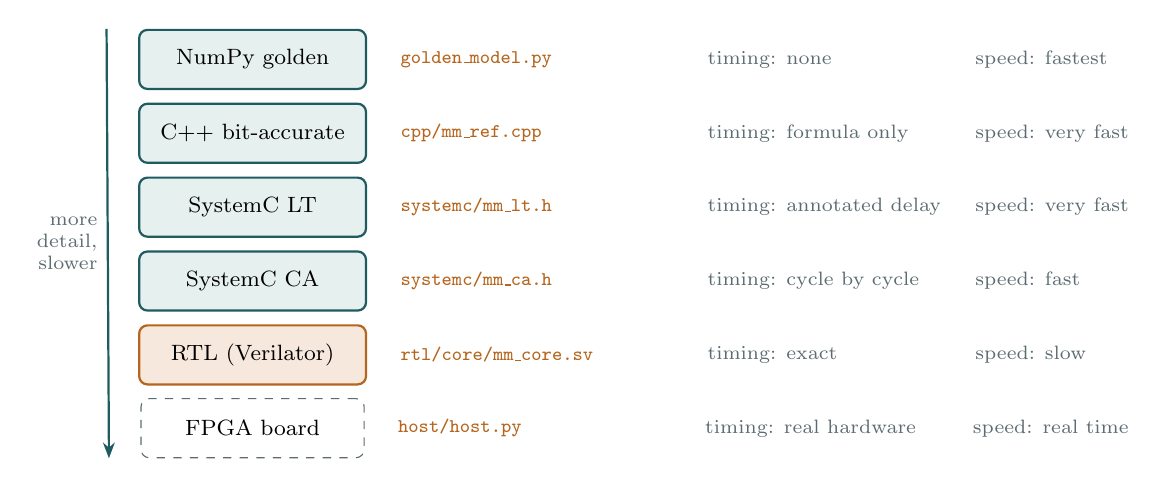
\begin{tikzpicture}[node distance=1.6mm]
    \tikzset{lvl/.style={mod, minimum height=7.5mm, text width=26mm}}
    \node[lvl] (np) {NumPy golden};
    \node[lvl, below=of np] (cpp) {C++ bit-accurate};
    \node[lvl, below=of cpp] (lt) {SystemC LT};
    \node[lvl, below=of lt] (ca) {SystemC CA};
    \node[hot, minimum height=7.5mm, text width=26mm, below=of ca] (rtl) {RTL (Verilator)};
    \node[ext, minimum height=7.5mm, text width=26mm, below=of rtl] (fpga) {FPGA board};
    \foreach \n/\a/\b/\c in {np/\file{golden\_model.py}/none/fastest, cpp/\file{cpp/mm\_ref.cpp}/formula only/very fast,
        lt/\file{systemc/mm\_lt.h}/annotated delay/very fast, ca/\file{systemc/mm\_ca.h}/cycle by cycle/fast,
        rtl/\file{rtl/core/mm\_core.sv}/exact/slow, fpga/\file{host/host.py}/real hardware/real time} {
      \node[anchor=west, font=\scriptsize] at ($(\n.east)+(3mm,0)$) {\a};
      \node[anchor=west, font=\scriptsize, text=muted] at ($(\n.east)+(42mm,0)$) {timing: \b};
      \node[anchor=west, font=\scriptsize, text=muted] at ($(\n.east)+(76mm,0)$) {speed: \c};
    }
    \draw[wireb] ($(np.north west)+(-4mm,0)$) -- node[left, font=\scriptsize, align=right, text=muted]{more\\detail,\\slower} ($(fpga.south west)+(-4mm,0)$);
  \end{tikzpicture}
  \vspace{1mm}

  \small Every level runs the \textbf{same jobs} and must produce the \textbf{same C} and the
  \textbf{same counters}. Each level adds detail; the fast levels are trusted only because they
  agree with the slow ones.
\end{frame}

% =====================================================================
\begin{frame}{How the files fit together}
  \centering
  \resizebox{0.98\textwidth}{!}{%
  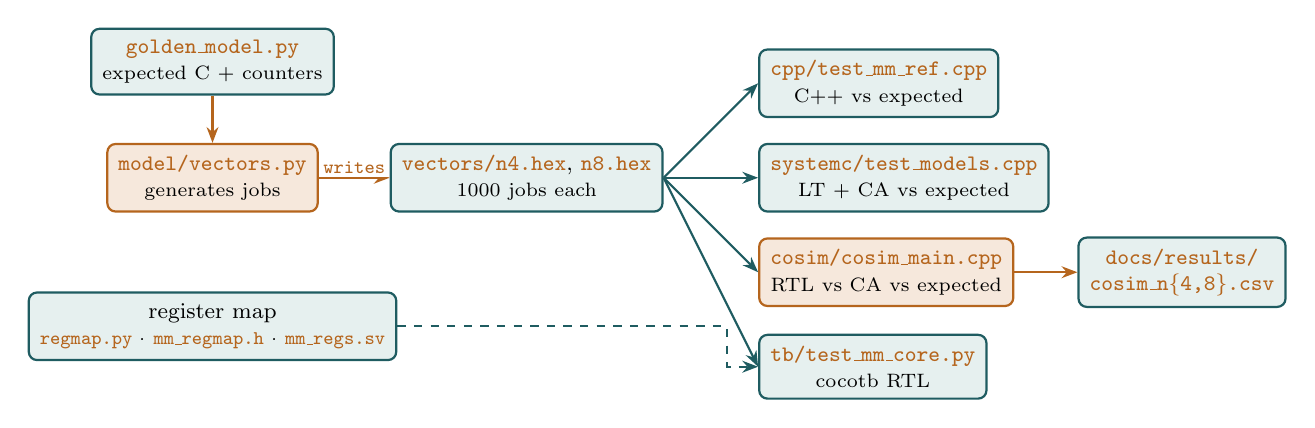
\begin{tikzpicture}[node distance=7mm and 9mm]
    \node[hot] (vec) {\file{model/vectors.py}\\\scriptsize generates jobs};
    \node[mod, right=of vec] (hex) {\file{vectors/n4.hex}, \file{n8.hex}\\\scriptsize 1000 jobs each};
    \node[mod, above=6mm of vec] (gold) {\file{golden\_model.py}\\\scriptsize expected C + counters};
    \node[mod, right=12mm of hex, yshift=12mm] (cpp) {\file{cpp/test\_mm\_ref.cpp}\\\scriptsize C++ vs expected};
    \node[mod, right=12mm of hex] (sc) {\file{systemc/test\_models.cpp}\\\scriptsize LT + CA vs expected};
    \node[hot, right=12mm of hex, yshift=-12mm] (co) {\file{cosim/cosim\_main.cpp}\\\scriptsize RTL vs CA vs expected};
    \node[mod, right=12mm of hex, yshift=-24mm] (tb) {\file{tb/test\_mm\_core.py}\\\scriptsize cocotb RTL};
    \node[mod, below=10mm of vec] (rm) {register map\\\scriptsize \file{regmap.py} \textperiodcentered{} \file{mm\_regmap.h} \textperiodcentered{} \file{mm\_regs.sv}};
    \node[mod, right=8mm of co] (csv) {\file{docs/results/}\\\file{cosim\_n\{4,8\}.csv}};
    \draw[wire] (gold) -- (vec);
    \draw[wire] (vec) -- node[lbl,above]{writes} (hex);
    \foreach \t in {cpp,sc,co,tb} \draw[wireb] (hex.east) -- (\t.west);
    \draw[wire] (co) -- (csv);
    \draw[wireb, dashed] (rm.east) -| ([xshift=-4mm]tb.west) -- (tb.west);
  \end{tikzpicture}}
  \vspace{1mm}

  \small\raggedright Two things are \textbf{shared by every level}: the test-vector files (same inputs,
  same expected outputs) and the register map (same addresses). That is what makes the levels
  comparable at all.
\end{frame}

% =====================================================================
\begin{frame}
  \centering\vspace{10mm}
  {\Large\bfseries\color{pcb} A.\ Shared test vectors and register map}\\[4mm]
  \color{muted} Before any model: agree on the inputs and the addresses
\end{frame}

% =====================================================================
\begin{frame}[fragile]{Shared test vectors: \file{model/vectors.py}}
  \begin{columns}[T]
    \column{0.47\textwidth}
    \begin{why}
      If every model made its own random inputs, a mismatch would not tell you \textbf{which}
      model is wrong. One shared file means any difference points at exactly one model.
    \end{why}
    \begin{how}
      \begin{itemize}
        \item 1000 jobs per N, fixed seed (reproducible).
        \item \textbf{20 edge-case jobs}: 5 patterns $\times$ K $\in$ \{1, 2N$-$2, 2N$-$1, 64\}.
        \item Then random A, B, \textbf{K $\in$ [1, 64]}.
        \item Expected C, counters: \file{golden\_model.py}.
      \end{itemize}
    \end{how}
    \column{0.5\textwidth}
    \small\textbf{File format}: 5 lines per job, all hex
\begin{lstlisting}
job 4 2           <- N=4, K=2
a 7f 80 01 ff ..  <- N*K int8, row-major
b 02 fe 7f 00 ..  <- K*N int8, row-major
c xxxxxxxx ..     <- N*N int32: expected C
p a 9 9 20        <- TOTAL=10 COMPUTE=9
                     FILLDRAIN=9 MACS=32
\end{lstlisting}
    \vspace{1mm}
    \footnotesize
    \begin{itemize}
      \item Why K = 2N$-$2 and 2N$-$1? They sit exactly on the boundary where
            \sig{all\_active} turns on, the easiest place for an off-by-one bug.
      \item Readers: \sig{read\_vectors()} in Python and in \file{mm\_ref.cpp}.
    \end{itemize}
  \end{columns}
\end{frame}

% =====================================================================
\begin{frame}{One register map, written three times}
  \begin{columns}[T]
    \column{0.47\textwidth}
    \begin{why}
      The same test sequence must run on the SystemC model and on the RTL pins. That only works
      if both agree on every address and bit. A model with a different map is testing a different
      design.
    \end{why}
    \begin{how}
      \begin{itemize}
        \item \file{model/regmap.py} --- Python (cocotb, host)
        \item \file{model/systemc/mm\_regmap.h} --- C++ / SystemC
        \item \file{rtl/core/mm\_regs.sv} --- the hardware
        \item One TLM transaction (4 bytes, byte address) = one RTL bus transaction.
      \end{itemize}
    \end{how}
    \column{0.5\textwidth}\scriptsize
    \resizebox{\linewidth}{!}{%
    \begin{tabular}{@{}l l l@{}}
      \toprule
      \textbf{Address} & \textbf{Name} & \textbf{Use in the models} \\
      \midrule
      0x0000 & CTRL & START / SOFT\_RESET \\
      0x0004 & STATUS & poll BUSY, DONE \\
      0x0008 & CFG\_K & set K \\
      0x000C & INFO & N, K\_MAX, VERSION \\
      0x0010 & PERF\_TOTAL & compared \\
      0x0014 & PERF\_COMPUTE & compared \\
      0x0018 & PERF\_FILLDRAIN & compared \\
      0x001C & PERF\_IDLE & \textbf{not} compared (host timing) \\
      0x0020 & PERF\_MACS & compared \\
      0x1000+ & A\_BUF & i$\cdot$K\_MAX + k \\
      0x2000+ & B\_BUF & k$\cdot$N + j \\
      0x3000+ & C\_BUF & 4(i$\cdot$N + j) \\
      \bottomrule
    \end{tabular}}
  \end{columns}
\end{frame}

% =====================================================================
\begin{frame}
  \centering\vspace{10mm}
  {\Large\bfseries\color{pcb} B.\ NumPy golden model, C++ model, analytical performance model}\\[4mm]
  \color{muted} What the right answer is, and how many cycles it should take
\end{frame}

% =====================================================================
\begin{frame}[fragile]{NumPy golden model: \file{model/golden\_model.py}}
  \begin{columns}[T]
    \column{0.47\textwidth}
    \begin{why}
      We need one reference that is \textbf{obviously correct}. NumPy's \sig{A @ B} is short enough
      to trust by reading it, and Python makes it easy to use from cocotb and the host script.
    \end{why}
    \begin{how}
      Multiply in 64-bit (never overflows for these sizes), then \textbf{wrap to 32 bits} the way
      the hardware accumulator does. \sig{expected\_perf()} gives every counter.
    \end{how}
    \column{0.5\textwidth}
\begin{lstlisting}[language=Python]
def matmul_int32(a, b):
    c = (np.asarray(a, np.int64)
         @ np.asarray(b, np.int64))
    # wrap to int32, like the hardware
    return (c + 2**31) % 2**32 - 2**31
\end{lstlisting}
    \scriptsize
    \textbf{Edge cases} (\sig{edge\_cases()}) and why each exists:\\[1mm]
    \begin{tabular}{@{}l l@{}}
      \toprule
      zeros & accumulators must stay 0 \\
      all\_min ($-$128$\cdot$$-$128) & largest positive sum \\
      all\_max (127$\cdot$127) & large positive sum \\
      min\_times\_max ($-$128$\cdot$127) & largest negative sum \\
      identity & C must equal B's rows \\
      \bottomrule
    \end{tabular}
  \end{columns}
\end{frame}

% =====================================================================
\begin{frame}[fragile]{C++ bit-accurate model: \file{model/cpp/mm\_ref.cpp}}
  \begin{columns}[T]
    \column{0.45\textwidth}
    \begin{why}
      \begin{itemize}
        \item Python cannot be linked into SystemC, Verilator or a UVM scoreboard; C++ can
              (UVM calls it through \textbf{DPI-C} in Phase~6).
        \item Much faster than Python for 1000s of jobs.
        \item \textbf{Bit-accurate}: same widths and overflow as \file{pe.sv}, so its output
              can be compared bit for bit.
      \end{itemize}
    \end{why}
    \column{0.52\textwidth}
\begin{lstlisting}[language=C++]
void matmul_ref(int n, int k, const int8_t* a,
                const int8_t* b, int32_t* c) {
  for (int i = 0; i < n; ++i)
    for (int j = 0; j < n; ++j) {
      uint32_t acc = 0;   // unsigned: defined wrap
      for (int kk = 0; kk < k; ++kk) {
        int16_t prod = int16_t(a[i*k + kk])
                     * int16_t(b[kk*n + j]);
        // sign-extend to 32 bits, add mod 2^32
        acc += uint32_t(int32_t(prod));
      }
      c[i*n + j] = int32_t(acc);
    }
}
\end{lstlisting}
    \begin{how}
      \footnotesize int8 $\times$ int8 $\to$ \textbf{int16} product (like \sig{prod} in pe.sv),
      sign-extended to 32 bits and added in \textbf{uint32}.
    \end{how}
  \end{columns}
\end{frame}

% =====================================================================
\begin{frame}{The C++ trap: why the accumulator is \sig{uint32\_t}}
  \begin{columns}[T]
    \column{0.5\textwidth}
    \begin{why}
      In C and C++, \textbf{signed integer overflow is undefined behaviour}. The compiler may
      assume it never happens and optimise in ways that give a \textbf{different} answer from
      hardware, which simply wraps.
    \end{why}
    \begin{how}
      Unsigned overflow \textbf{is} defined: it wraps modulo $2^{32}$, exactly like a 32-bit
      hardware adder. So: add as \sig{uint32\_t}, convert back to \sig{int32\_t} at the end.
    \end{how}
    \column{0.47\textwidth}\small
    \textbf{Does it ever overflow here?}
    \begin{itemize}
      \item Largest product: $(-128)\times(-128) = 16\,384$ (fits int16: max 32\,767).
      \item K = 64: $64 \times 16\,384 = 1\,048\,576$ --- fits int32 easily.
      \item So with K $\le$ 64 it never overflows.
    \end{itemize}
    \textbf{Then why bother?} The model must follow the \textbf{spec} (``32-bit wrap''), not the
    test sizes. If K\_MAX is raised later, the model is still correct.\\[2mm]
    \footnotesize\color{muted} Interview line: ``the reference model mirrors the spec, not the RTL code ---
    otherwise both can share the same bug.''
  \end{columns}
\end{frame}

% =====================================================================
\begin{frame}{Analytical performance model: \sig{predict\_perf()}}
  \begin{columns}[T]
    \column{0.42\textwidth}
    \begin{why}
      Before running anything, we want a \textbf{prediction}: how many cycles should a job take?
      That prediction is the target the CA model, the RTL and the FPGA are all checked against.
    \end{why}
    \begin{how}
      Count the controller states: 1 CLEAR + K COMPUTE + (2N$-$1) DRAIN. All N$^2$ PEs are busy
      only for steps 2N$-$1 \ldots{} K.
    \end{how}
    \column{0.55\textwidth}\scriptsize
    \begin{tabular}{@{}l l@{}}
      \toprule
      \textbf{Counter} & \textbf{Formula} \\
      \midrule
      total & K + 2N \\
      compute & K + 2N $-$ 1 \\
      filldrain & compute $-$ max(0, K $-$ 2N + 2) \\
      macs & N$^2\cdot$K \\
      utilisation & macs / (N$^2\cdot$compute) \\
      \bottomrule
    \end{tabular}\\[2mm]
    \begin{tabular}{@{}c c c c c c c@{}}
      \toprule
      \textbf{N} & \textbf{K} & \textbf{total} & \textbf{compute} & \textbf{fill/drain} & \textbf{util.} & \textbf{GOPS} \\
      \midrule
      4 & 16 & 24 & 23 & 13 & 69.6\,\% & 1.07 \\
      4 & 64 & 72 & 71 & 13 & 90.1\,\% & 1.42 \\
      8 & 16 & 32 & 31 & 29 & 51.6\,\% & 3.20 \\
      8 & 64 & 80 & 79 & 29 & 81.0\,\% & 5.12 \\
      \bottomrule
    \end{tabular}\\[1mm]
    \color{muted} GOPS = 2$\cdot$macs / (total / 50\,MHz). Full table (N $\in$ \{4,8\}, K = 1..64):
    \file{docs/results/perf\_model.csv} from \file{perf\_table.cpp}.
  \end{columns}
\end{frame}

% =====================================================================
\begin{frame}[fragile]{First check: C++ model == NumPy (\file{test\_mm\_ref.cpp})}
  \begin{columns}[T]
    \column{0.5\textwidth}
\begin{lstlisting}[language=C++]
for (const mm::Job& j : mm::read_vectors(file)) {
  std::vector<int32_t> c(j.n * j.n);
  mm::matmul_ref(j.n, j.k, j.a.data(),
                 j.b.data(), c.data());
  bool ok = (c == j.c) &&
    (mm::predict_perf(j.n, j.k) == j.perf);
  ...
}
\end{lstlisting}
    \centering
    \begin{tcolorbox}[colback=coppert,colframe=copper,arc=2mm,width=0.9\linewidth,halign=center]
      \Large\bfseries 2000 / 2000\\[-1mm]\scriptsize\mdseries vectors match (C and counters)
    \end{tcolorbox}
    \column{0.47\textwidth}
    \begin{why}
      Two references written in two languages by two methods. If they agree on 2000 jobs, a bug in
      either one is very unlikely. Only then do we use them to judge the SystemC models and RTL.
    \end{why}
    \begin{how}
      Read every job from \sig{n4.hex} and \sig{n8.hex}, compute C and the predicted counters, compare
      with what NumPy wrote. \sig{make -C model/cpp test}.
    \end{how}
  \end{columns}
\end{frame}

% =====================================================================
\begin{frame}
  \centering\vspace{10mm}
  {\Large\bfseries\color{pcb} C.\ SystemC: loosely-timed (LT) and cycle-approximate (CA) models}\\[4mm]
  \color{muted} Models of the whole accelerator, with a register interface and a notion of time
\end{frame}

% =====================================================================
\begin{frame}{Why SystemC, and the TLM-2.0 pieces we use}
  \begin{columns}[T]
    \column{0.47\textwidth}
    \begin{why}
      \begin{itemize}
        \item The C++ model only computes C. A real model of the accelerator also needs
              \textbf{registers, a bus, time and a clock}.
        \item SystemC is a C++ library (IEEE 1666) that adds exactly that: modules, ports,
              clocks, simulated time.
        \item It is the standard language for architecture models and virtual platforms.
      \end{itemize}
    \end{why}
    \column{0.5\textwidth}
    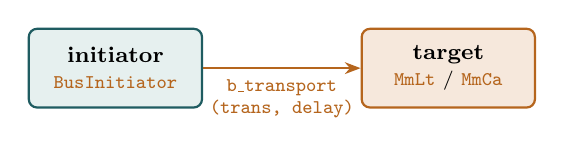
\begin{tikzpicture}[node distance=5mm and 10mm]
      \node[mod, minimum width=22mm, minimum height=10mm] (ini) {\textbf{initiator}\\\scriptsize \file{BusInitiator}};
      \node[hot, right=20mm of ini, minimum width=22mm, minimum height=10mm] (tgt) {\textbf{target}\\\scriptsize \file{MmLt} / \file{MmCa}};
      \draw[wire] (ini) -- node[lbl,below=1mm,align=center]{b\_transport\\(trans, delay)} (tgt);
    \end{tikzpicture}\\[3mm]
    \begin{how}
      \begin{itemize}
        \item \textbf{Socket}: initiator socket (bus master) bound to a target socket (the model).
        \item \textbf{Generic payload} = one transaction: command (read/write), address, 4-byte data
              pointer, length, response status.
        \item \textbf{b\_transport}: a blocking function call. The target does the access and adds
              its latency to \sig{delay}.
      \end{itemize}
    \end{how}
  \end{columns}
\end{frame}

% =====================================================================
\begin{frame}[fragile]{Shared state for both models: \file{mm\_state.h}}
  \begin{columns}[T]
    \column{0.47\textwidth}
    \begin{why}
      LT and CA must decode registers \textbf{identically}: same ignored writes, same reset values.
      Writing the decode once means the two models cannot drift apart. Only \textbf{timing} differs
      between them.
    \end{why}
    \begin{how}
      \sig{MmState} holds the buffers, CFG\_K, BUSY/DONE and counters, with the RTL's rules:
      \begin{itemize}
        \item A/B writes ignored while BUSY; low byte stored.
        \item Bad CFG\_K and START-while-BUSY ignored.
        \item Unmapped reads return 0.
      \end{itemize}
    \end{how}
    \column{0.5\textwidth}
\begin{lstlisting}[language=C++]
enum class WriteEffect { NONE, START, SOFT_RESET };

WriteEffect write(uint16_t addr, uint32_t d) {
  int region = addr >> 12, off = addr & 0xFFF;
  if (region == 0) {
    if (addr == CTRL) {
      if (d & SOFT_RESET) return SOFT_RESET;
      if ((d & START) && !busy) return START;
    } else if (addr == CFG_K && d >= 1
               && d <= k_max)
      cfg_k = d;
  } else if (!busy && region == 1
             && off < n * k_max)
    a[off] = int8_t(d & 0xFF);
  ...                       // B: region 2
  return NONE;
}
\end{lstlisting}
    \footnotesize The \textbf{model} decides \emph{when} a START or SOFT\_RESET takes effect;
    \sig{write()} only reports it.
  \end{columns}
\end{frame}

% =====================================================================
\begin{frame}{Loosely-timed model: \file{mm\_lt.h}}
  \begin{columns}[T]
    \column{0.45\textwidth}
    \begin{why}
      The fastest model that still looks like the accelerator from outside: good for many jobs,
      for software, and as the first check of register behaviour.
    \end{why}
    \begin{how}
      \begin{itemize}
        \item No clock. On START: compute C \textbf{at once}, take counters from
              \sig{predict\_perf()}, set \sig{done\_at = now + total$\cdot$20\,ns}.
        \item STATUS reads BUSY until time passes \sig{done\_at}.
        \item Each access adds one bus cycle to \sig{delay}.
      \end{itemize}
    \end{how}
    \column{0.52\textwidth}
    \centering
    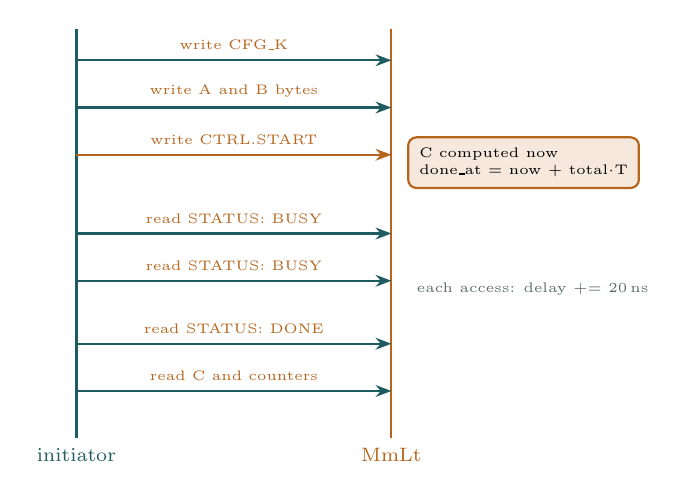
\begin{tikzpicture}[x=1mm,y=1mm]
      \draw[thick, pcbmid] (0,0) -- (0,-52) node[below, font=\scriptsize]{initiator};
      \draw[thick, copper] (40,0) -- (40,-52) node[below, font=\scriptsize]{MmLt};
      \foreach \y/\t/\c in {-4/write CFG\_K/pcbmid, -10/write A and B bytes/pcbmid,
                            -16/write CTRL.START/copper, -26/read STATUS: BUSY/pcbmid,
                            -32/read STATUS: BUSY/pcbmid, -40/read STATUS: DONE/pcbmid,
                            -46/read C and counters/pcbmid}
        \draw[wire, draw=\c] (0,\y) -- node[above, font=\tiny]{\t} (40,\y);
      \node[hot, font=\tiny, anchor=west, align=left] at (42,-17) {C computed now\\done\_at = now + total$\cdot$T};
      \node[font=\tiny, text=muted, anchor=west] at (42,-33) {each access: delay += 20\,ns};
    \end{tikzpicture}\\[1mm]
    \footnotesize\raggedright\textbf{Temporal decoupling:} the LT test thread never waits per access;
    it only accumulates \sig{delay} and syncs \textbf{once} at the end. That is what makes LT fast.
  \end{columns}
\end{frame}

% =====================================================================
\begin{frame}[fragile]{Cycle-approximate model: \file{mm\_ca.h}}
  \begin{columns}[T]
    \column{0.47\textwidth}
    \begin{why}
      LT only \emph{predicts} cycles from a formula. CA \textbf{counts} them, running the same
      FSM as \file{mm\_controller.sv} and counter rules as \file{mm\_regs.sv}. A wrong formula
      shows up as a disagreement.
    \end{why}
    \begin{how}
      \begin{itemize}
        \item \sig{SC\_THREAD} wakes on every rising edge.
        \item Counters use the state \textbf{before} the edge.
        \item START takes effect at the \textbf{next edge}.
        \item C is computed functionally at DONE.
      \end{itemize}
    \end{how}
    \column{0.52\textwidth}
\begin{lstlisting}[language=C++]
for (;;) {
  wait();                        // rising edge
  bool en  = (st == COMPUTE || st == DRAIN);
  bool all = en && t >= 2*n-1 && t <= K;
  // counters: same rules as mm_regs.sv
  if (busy && st != DONE) ++total;
  if (en)                 ++compute;
  if (en && !all)         ++filldrain;
  if (st == COMPUTE)      macs += n*n;
  // FSM: same as mm_controller.sv
  switch (st) {
  case IDLE:    if (start) st = CLEAR; break;
  case CLEAR:   t = 0; st = COMPUTE;   break;
  case COMPUTE: if (t == K-1) st = DRAIN;
                ++t;                   break;
  case DRAIN:   if (t == K+2*n-2) {
                  compute_c(); st = DONE;
                } else ++t;            break;
  case DONE:    done = true; st = IDLE;
  }
}
\end{lstlisting}
  \end{columns}
\end{frame}

% =====================================================================
\begin{frame}{LT vs CA vs RTL: what each one models}
  \centering\small
  \begin{tabular}{@{}l c c c@{}}
    \toprule
    & \textbf{SystemC LT} & \textbf{SystemC CA} & \textbf{RTL} \\
    \midrule
    Register map and access rules & \checkmark & \checkmark & \checkmark \\
    Result C & \checkmark{} (at START) & \checkmark{} (at DONE) & \checkmark{} (accumulates) \\
    Clock & no & yes & yes \\
    Controller FSM, cycle by cycle & no & \checkmark & \checkmark \\
    Counters & from the formula & counted each cycle & counted each cycle \\
    Datapath pipeline (skew, PEs) & no & no & \checkmark \\
    RAM contents over time & no & no & \checkmark \\
    Reading C in the middle of a job & old result & old result & partial sums \\
    PERF\_IDLE & approximate & approximate & exact \\
    Speed & fastest & fast & slow \\
    \bottomrule
  \end{tabular}\\[3mm]
  \raggedright\small
  \begin{itemize}
    \item \textbf{Why this matters:} knowing what a model does \emph{not} model is as important as
          what it does. That is why PERF\_IDLE (depends on host timing) is excluded from comparisons.
  \end{itemize}
\end{frame}

% =====================================================================
\begin{frame}[fragile]{One job sequence for every level: \sig{run\_job()} in \file{bus\_initiator.h}}
  \begin{columns}[T]
    \column{0.52\textwidth}
\begin{lstlisting}[language=C++]
// simplified from bus_initiator.h
template <class Bus, class Tick>
void run_job(Bus& bus, const Job& j, ...,
             Tick tick) {
  bus.write(CFG_K, j.k);              tick();
  for (i, kk)  bus.write(a_addr(i, kk), A[i][kk]);
  for (kk, jj) bus.write(b_addr(kk, jj), B[kk][jj]);
  bus.write(CTRL, CTRL_START);        tick();
  while (!(bus.read(STATUS) & DONE))  tick();
  for (idx)    c[idx] = bus.read(C_BUF + 4*idx);
  p = { bus.read(PERF_TOTAL), bus.read(PERF_COMPUTE),
        bus.read(PERF_FILLDRAIN), bus.read(PERF_MACS) };
}
\end{lstlisting}
    \column{0.45\textwidth}
    \begin{why}
      If each level had its own test sequence, a difference could come from the
      \textbf{test}, not the design. One sequence removes that doubt.
    \end{why}
    \begin{how}
      A C++ template: \sig{Bus} is anything with \sig{write()} / \sig{read()}:
      \begin{itemize}
        \item \sig{BusInitiator} $\to$ TLM socket $\to$ LT or CA model
        \item \sig{RtlBus} $\to$ real pins of the verilated RTL
      \end{itemize}
      \sig{Tick} decides how time passes between accesses (nothing for LT, one clock for CA).
    \end{how}
  \end{columns}
\end{frame}

% =====================================================================
\begin{frame}{Second check: SystemC models (\file{test\_models.cpp})}
  \begin{columns}[T]
    \column{0.5\textwidth}
    \begin{how}
      \begin{itemize}
        \item One SystemC top: a 20\,ns \sig{sc\_clock}, one LT model, one CA model, two initiators.
        \item Two threads run all 1000 jobs: \sig{run\_lt} (no waiting) and \sig{run\_ca}
              (drives on the falling edge).
        \item Each job: C and the 4 counters must equal the vector file.
        \item CA also \textbf{times a bare restart} with the clock, independently of the counters,
              and compares it to \sig{predict\_perf()}.
      \end{itemize}
    \end{how}
    \scriptsize\color{muted} Measured $-$ 2 = PERF\_TOTAL: START is seen one edge later, and the
    DONE cycle is not counted.
    \column{0.47\textwidth}
    \centering\small
    \resizebox{\linewidth}{!}{%
    \begin{tabular}{@{}l c@{}}
      \toprule
      \textbf{Check (2 $\times$ 1000 jobs)} & \textbf{Result} \\
      \midrule
      LT: C + counters & 0 mismatches \\
      CA: C + counters & 0 mismatches \\
      CA: measured vs predicted cycles & \textbf{0 cycles} error \\
      \bottomrule
    \end{tabular}}\\[3mm]
    \begin{why}
      Target was $\pm$2 cycles. Getting \textbf{0} shows the CA model reproduces the controller
      exactly, so it can now be used as the reference for the RTL.
    \end{why}
  \end{columns}
\end{frame}

% =====================================================================
\begin{frame}
  \centering\vspace{10mm}
  {\Large\bfseries\color{pcb} D.\ RTL and SystemC model running side by side}\\[4mm]
  \color{muted} \file{cosim/cosim\_main.cpp} + Verilator
\end{frame}

% =====================================================================
\begin{frame}{Why co-simulation?}
  \begin{columns}[T]
    \column{0.5\textwidth}
    \begin{why}
      \begin{itemize}
        \item cocotb already checks the RTL's \textbf{answers}. Co-sim also checks its
              \textbf{timing and counters} against an independent model, job by job.
        \item It proves the model and the RTL describe the \textbf{same machine}, so the model
              can be trusted for performance studies.
        \item It catches bugs where the answer is right but the behaviour is wrong
              (see the mutation test).
      \end{itemize}
    \end{why}
    \column{0.47\textwidth}\small
    \textbf{What is compared, every job}
    \begin{enumerate}
      \item \textbf{C}: RTL = CA model = expected
      \item \textbf{Counters}: RTL = CA model = analytical prediction
      \item \textbf{START $\to$ DONE at the pins}: measured from the \sig{done} signal, without using
            the counters
    \end{enumerate}
    \vspace{2mm}
    \footnotesize\color{muted} Item 3 matters: if the counters themselves had a bug, comparing
    counters with counters could hide it. Timing the pins is an independent check.
  \end{columns}
\end{frame}

% =====================================================================
\begin{frame}[fragile]{Verilator: turning RTL into a SystemC module}
  \begin{columns}[T]
    \column{0.47\textwidth}
    \begin{why}
      SystemC cannot read SystemVerilog. Verilator \textbf{compiles} the RTL into C++; with
      \sig{--sc} it becomes an \sig{sc\_module} with \sig{sc\_in}/\sig{sc\_out} ports, so RTL and
      model live in the \textbf{same simulation} and share one clock.
    \end{why}
    \begin{how}
      \begin{itemize}
        \item Cycle-based and 2-state (no X/Z) $\to$ very fast.
        \item \sig{-GN=4} / \sig{-GN=8} sets the top parameter, so one harness covers both sizes.
        \item Output: class \sig{Vmm\_core} with the same ports as \file{mm\_core.sv}.
      \end{itemize}
    \end{how}
    \column{0.5\textwidth}
    \footnotesize\textbf{From \file{cosim/Makefile}}
\begin{lstlisting}
# simplified
verilator --sc --exe --build -j 0 \
  -GN=$(N) -GK_MAX=64 \
  --top-module mm_core \
  --Mdir build/n$(N) \
  rtl/core/pe.sv \
  rtl/core/systolic_array.sv \
  rtl/core/skew_buffer.sv \
  rtl/core/sram_sp.sv \
  rtl/core/mm_controller.sv \
  rtl/core/mm_regs.sv rtl/core/mm_core.sv \
  cosim_main.cpp model/cpp/mm_ref.cpp
\end{lstlisting}
    \vspace{1mm}
    \footnotesize Only \file{rtl/core/} is compiled: the co-sim drives \sig{mm\_core}'s register
    bus directly, without the UART.
  \end{columns}
\end{frame}

% =====================================================================
\begin{frame}{Co-simulation architecture (\file{cosim\_main.cpp})}
  \centering
  \resizebox{0.96\textwidth}{!}{%
  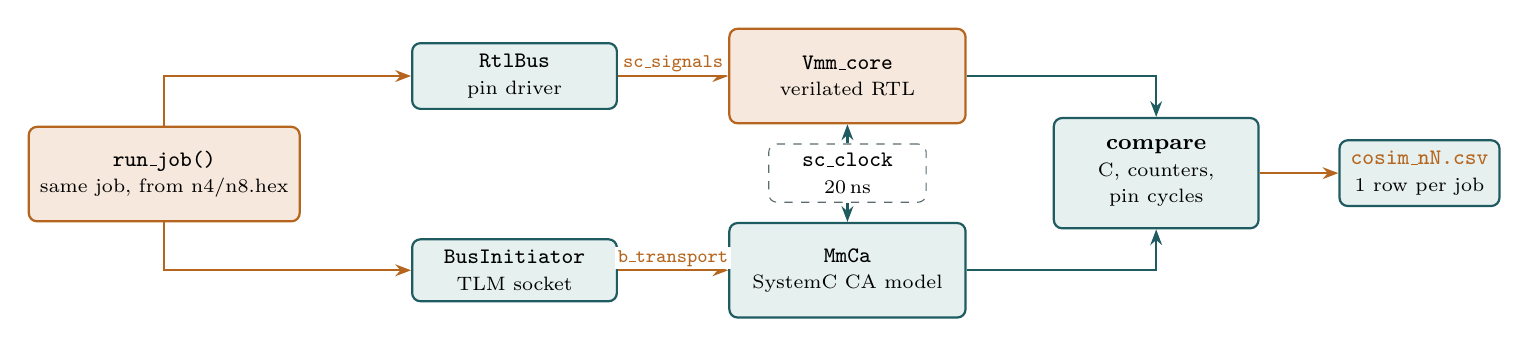
\begin{tikzpicture}[node distance=8mm and 12mm]
    \node[hot, minimum width=28mm, minimum height=12mm] (job) {\sig{run\_job()}\\\scriptsize same job, from n4/n8.hex};
    \node[mod, above right=2mm and 14mm of job, minimum width=26mm] (rb) {\sig{RtlBus}\\\scriptsize pin driver};
    \node[mod, below right=2mm and 14mm of job, minimum width=26mm] (ib) {\sig{BusInitiator}\\\scriptsize TLM socket};
    \node[hot, right=14mm of rb, minimum width=30mm, minimum height=12mm] (rtl) {\sig{Vmm\_core}\\\scriptsize verilated RTL};
    \node[mod, right=14mm of ib, minimum width=30mm, minimum height=12mm] (ca) {\sig{MmCa}\\\scriptsize SystemC CA model};
    \node[ext, minimum width=20mm] (clk) at ($(rtl)!0.5!(ca)+(0,0)$) {\sig{sc\_clock}\\\scriptsize 20\,ns};
    \node[mod, right=16mm of clk, minimum width=26mm, minimum height=14mm] (cmp) {\textbf{compare}\\\scriptsize C, counters,\\\scriptsize pin cycles};
    \node[mod, right=10mm of cmp] (csv) {\file{cosim\_nN.csv}\\\scriptsize 1 row per job};
    \draw[wire] (job) |- (rb);
    \draw[wire] (job) |- (ib);
    \draw[wire] (rb) -- node[lbl,above]{sc\_signals} (rtl);
    \draw[wire] (ib) -- node[lbl,above]{b\_transport} (ca);
    \draw[wireb, dashed] (clk) -- (rtl);
    \draw[wireb, dashed] (clk) -- (ca);
    \draw[wireb] (rtl.east) -| (cmp.north);
    \draw[wireb] (ca.east) -| (cmp.south);
    \draw[wire] (cmp) -- (csv);
  \end{tikzpicture}}
  \vspace{2mm}
  \raggedright\small
  \begin{itemize}
    \item One \sig{SC\_MODULE Cosim} holds everything: the clock, the RTL with its signals, the CA
          model, both bus drivers, the job list.
    \item One \sig{SC\_THREAD run()}: reset the RTL for 3 cycles, then for each job run it on the RTL,
          run it on the model, time a restart at the pins, compare, write a CSV row.
  \end{itemize}
\end{frame}

% =====================================================================
\begin{frame}[fragile]{Driving the RTL pins: \sig{RtlBus}}
  \begin{columns}[T]
    \column{0.5\textwidth}
\begin{lstlisting}[language=C++]
void request(bool wr, uint16_t a, uint32_t d) {
  valid.write(true); write_en.write(wr);
  addr.write(a);     wdata.write(d);
  for (;;) {
    wait(SC_ZERO_TIME);         // settle
    bool rdy = ready.read();
    wait(clk.negedge_event());  // next fall
    if (rdy) break;             // accepted
  }
  valid.write(false);
}
uint32_t read(uint16_t a) {
  request(false, a, 0);
  if (!rvalid.read())           // 1 cycle
    throw std::runtime_error(...);
  return rdata.read();
}
\end{lstlisting}
    \column{0.47\textwidth}
    \begin{why}
      Signals driven exactly at a rising edge race with the RTL's flip-flops. Driving on the
      \textbf{falling} edge and sampling mid-cycle avoids the race.
    \end{why}
    \begin{how}
      \begin{itemize}
        \item Drive on the falling edge; the RTL samples on the rising edge.
        \item Hold \sig{bus\_valid} until \sig{bus\_ready} was seen.
        \item A read \textbf{must} see \sig{bus\_rvalid} one cycle later, so the protocol
              is checked too (same rule as cocotb).
      \end{itemize}
    \end{how}
  \end{columns}
\end{frame}

% =====================================================================
\begin{frame}{Measuring cycles at the pins}
  \begin{columns}[T]
    \column{0.52\textwidth}
    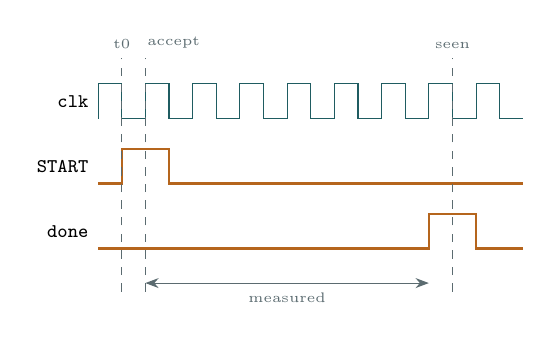
\begin{tikzpicture}[x=6mm,y=5.5mm, font=\scriptsize\ttfamily]
      \node[left] at (0,4) {clk};
      \foreach \t in {0,...,8} \draw[pcbmid] (\t,3.6) -- (\t,4.4) -- (\t+0.5,4.4) -- (\t+0.5,3.6) -- (\t+1,3.6);
      \node[left] at (0,2.5) {START};
      \draw[copper,thick] (0,2.1) -- (0.5,2.1) -- (0.5,2.9) -- (1.5,2.9) -- (1.5,2.1) -- (9,2.1);
      \node[left] at (0,1) {done};
      \draw[copper,thick] (0,0.6) -- (7,0.6) -- (7,1.4) -- (8,1.4) -- (8,0.6) -- (9,0.6);
      \draw[dashed,muted] (0.5,-0.4) -- (0.5,5) node[above,font=\tiny]{t0};
      \draw[dashed,muted] (1,-0.4) -- (1,5) node[above right,font=\tiny,xshift=-1mm]{accept};
      \draw[dashed,muted] (7.5,-0.4) -- (7.5,5) node[above,font=\tiny]{seen};
      \draw[{Stealth}-{Stealth},muted] (1,-0.2) -- node[below,font=\tiny]{measured} (7,-0.2);
    \end{tikzpicture}
    \column{0.45\textwidth}
    \begin{why}
      Counters are themselves hardware under test. Timing the \sig{done} pin gives a number that
      does \textbf{not} depend on the counter logic.
    \end{why}
    \begin{how}
      \begin{itemize}
        \item t0 = falling edge where START is driven.
        \item START is accepted at the next rising edge: $-T/2$.
        \item \sig{done} is seen at a falling edge: $-T/2$.
        \item \sig{pin\_cycles = (now $-$ t0 $-$ T) / T}, compared with \sig{predict\_perf().total}.
      \end{itemize}
    \end{how}
  \end{columns}
\end{frame}

% =====================================================================
\begin{frame}{Results: \file{docs/results/cosim\_n4.csv}, \file{cosim\_n8.csv}}
  \begin{columns}[T]
    \column{0.5\textwidth}
    \centering
    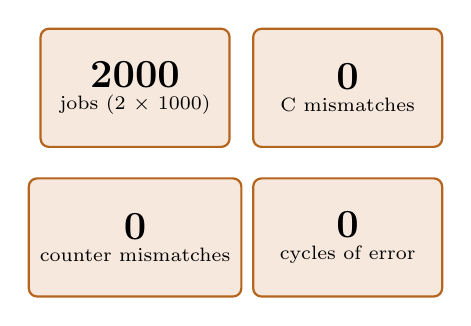
\begin{tikzpicture}
      \tikzset{stat/.style={hot, minimum width=24mm, minimum height=15mm, align=center}}
      \node[stat] at (0,0)   {\Large\bfseries 2000\\[-0.5mm]\scriptsize\mdseries jobs (2 $\times$ 1000)};
      \node[stat] at (2.7,0) {\Large\bfseries 0\\[-0.5mm]\scriptsize\mdseries C mismatches};
      \node[stat] at (0,-1.9)   {\Large\bfseries 0\\[-0.5mm]\scriptsize\mdseries counter mismatches};
      \node[stat] at (2.7,-1.9) {\Large\bfseries 0\\[-0.5mm]\scriptsize\mdseries cycles of error};
    \end{tikzpicture}
    \column{0.47\textwidth}\scriptsize
    \textbf{Sample rows} (RTL = CA = predicted)\\[1mm]
    \begin{tabular}{@{}c c c c c c@{}}
      \toprule
      \textbf{N} & \textbf{K} & \textbf{total} & \textbf{compute} & \textbf{fill/drain} & \textbf{pin cycles} \\
      \midrule
      8 & 1  & 17 & 16 & 16 & 17 \\
      8 & 64 & 80 & 79 & 29 & 80 \\
      4 & 64 & 72 & 71 & 13 & 72 \\
      \bottomrule
    \end{tabular}\\[2mm]
    \small
    CSV columns: job, N, K, predicted\_total, rtl/ca total, compute, filldrain, macs,
    rtl\_pin\_cycles, cycle\_error, c\_match.\\[1mm]
    \footnotesize\color{muted} K = 1 shows the extreme: with K $<$ 2N$-$1 the array is never fully
    busy, so every enabled cycle is fill/drain.
  \end{columns}
\end{frame}

% =====================================================================
\begin{frame}{Proving the harness works: a mutation test}
  \begin{columns}[T]
    \column{0.5\textwidth}
    \begin{why}
      ``0 mismatches'' is only meaningful if the harness \textbf{can} find a mismatch. A broken
      checker that always says PASS would also report 0.
    \end{why}
    \begin{how}
      Inject one deliberate bug in the RTL, rerun, confirm it is caught, then undo it:\\[1mm]
      \file{mm\_controller.sv}: the ``all PEs active'' bound \sig{2N-1} $\to$ \sig{2N-2}.
    \end{how}
    \column{0.47\textwidth}\small
    \textbf{What happened}
    \begin{itemize}
      \item C was still \textbf{correct} (the bug only affects a status signal).
      \item Co-sim immediately reported \textbf{PERF\_FILLDRAIN mismatches}.
    \end{itemize}
    \begin{tcolorbox}[colback=coppert,colframe=copper,arc=2mm]
      \small A check of answers alone would have \textbf{passed}. Performance correlation caught a
      real bug that functional checking missed.
    \end{tcolorbox}
    \footnotesize\color{muted} Good interview story: ``how do you know your checker works?''
  \end{columns}
\end{frame}

% =====================================================================
\begin{frame}{What co-simulation does not prove (yet)}
  \begin{columns}[T]
    \column{0.5\textwidth}\small
    \textbf{Limits}
    \begin{itemize}
      \item The CA model does not model the \textbf{datapath} (skew, PE pipeline, RAM timing). The
            RTL's C is checked against the expected values instead.
      \item Verilator is \textbf{2-state}: uninitialised (X) values are not visible.
      \item \textbf{PERF\_IDLE} is excluded: it depends on how fast the host polls.
      \item Simulation says nothing about \textbf{FPGA timing} (Fmax, slack) or the real UART link.
    \end{itemize}
    \column{0.47\textwidth}\small
    \textbf{Next steps that close these gaps}
    \begin{itemize}
      \item \textbf{Phase 4 --- FPGA:} read the same counters from the board over UART
            $\to$ model vs RTL vs \textbf{real hardware}.
      \item \textbf{Phase 6 --- UVM:} a 4-state simulator (Questa), constrained-random jobs,
            a DPI-C scoreboard calling \sig{matmul\_ref()}, functional coverage.
      \item \textbf{Correlation report:} predicted vs RTL vs FPGA cycles, error \%.
    \end{itemize}
  \end{columns}
\end{frame}

% =====================================================================
\begin{frame}[fragile]{Running it on Ubuntu, and the reading order}
  \begin{columns}[T]
    \column{0.5\textwidth}
\begin{lstlisting}
conda activate fpga         # tools
python3 model/vectors.py    # n4/n8.hex
make -C model/cpp test      # C++==NumPy
make -C model/systemc test  # LT + CA
make -C cosim               # RTL vs CA
# results: docs/results/cosim_n{4,8}.csv
\end{lstlisting}
    \footnotesize\color{muted} Run these on Ubuntu (the toolchain lives in the \sig{fpga} conda
    environment).
    \column{0.47\textwidth}\scriptsize
    \resizebox{\linewidth}{!}{%
    \begin{tabular}{@{}c l l@{}}
      \toprule
      \textbf{\#} & \textbf{Read} & \textbf{Focus} \\
      \midrule
      1 & golden\_model.py & matmul\_int32, expected\_perf \\
      2 & vectors.py & file format, edge cases \\
      3 & cpp/mm\_ref.cpp & uint32 wrap, predict\_perf \\
      4 & systemc/mm\_state.h & register decode \\
      5 & systemc/mm\_lt.h & b\_transport, done\_at \\
      6 & systemc/mm\_ca.h & clocked FSM, counters \\
      7 & systemc/bus\_initiator.h & run\_job template \\
      8 & systemc/test\_models.cpp & two threads, timing check \\
      9 & cosim/cosim\_main.cpp & RtlBus, compare, CSV \\
      10 & docs/results/phase5\_models.md & numbers + limits \\
      \bottomrule
    \end{tabular}}\\[2mm]
    \small\textbf{Exercise:} redo the mutation test yourself, then undo it.
  \end{columns}
\end{frame}

% =====================================================================
\begin{frame}{Interview questions on this part}
  \scriptsize
  \begin{columns}[T]
    \column{0.5\textwidth}
    \begin{enumerate}
      \item \textbf{Why a C++ model if you have NumPy?} It links into SystemC, Verilator and a UVM
            scoreboard (DPI-C), and it is fast.
      \item \textbf{What does bit-accurate mean?} Same widths and overflow as the RTL, so outputs match
            bit for bit.
      \item \textbf{Why \sig{uint32\_t} for the accumulator?} Signed overflow is undefined in C++;
            unsigned wraps like hardware.
      \item \textbf{LT vs CA?} LT: no clock, blocking calls, latency annotated, fastest. CA: clocked,
            counts cycles, follows the FSM.
      \item \textbf{What is temporal decoupling?} The initiator runs ahead, accumulating delay, and
            syncs rarely.
    \end{enumerate}
    \column{0.48\textwidth}
    \begin{enumerate}\setcounter{enumi}{5}
      \item \textbf{How do you co-simulate RTL with SystemC?} \sig{verilator --sc} makes the RTL an
            sc\_module; one clock, same job sequence, compare.
      \item \textbf{Why drive on the falling edge?} Avoids races with flip-flops at the rising edge.
      \item \textbf{How do you measure cycles independently?} Time START $\to$ \sig{done} at the pins.
      \item \textbf{How do you know the checker works?} Mutation test: inject a bug, see it caught.
      \item \textbf{What does your CA model not model?} The datapath pipeline and RAM timing; and
            PERF\_IDLE is excluded.
    \end{enumerate}
  \end{columns}
\end{frame}

% =====================================================================
\begin{frame}{Key takeaways}
  \centering
  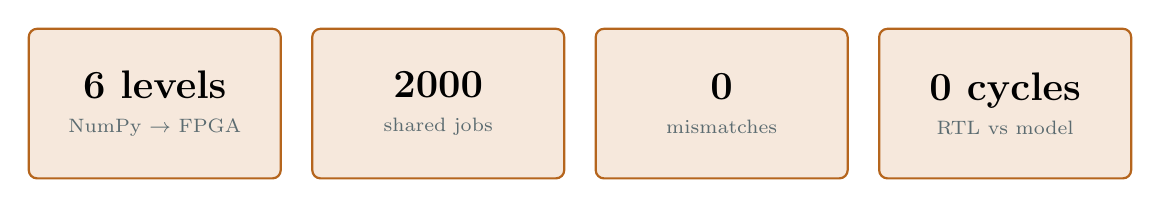
\begin{tikzpicture}
    \tikzset{stat/.style={hot, minimum width=32mm, minimum height=19mm, align=center}}
    \node[stat] at (0,0)    {\Large\bfseries 6 levels\\[1mm]\scriptsize\mdseries\color{muted} NumPy $\to$ FPGA};
    \node[stat] at (3.6,0)  {\Large\bfseries 2000\\[1mm]\scriptsize\mdseries\color{muted} shared jobs};
    \node[stat] at (7.2,0)  {\Large\bfseries 0\\[1mm]\scriptsize\mdseries\color{muted} mismatches};
    \node[stat] at (10.8,0) {\Large\bfseries 0 cycles\\[1mm]\scriptsize\mdseries\color{muted} RTL vs model};
  \end{tikzpicture}
  \vspace{5mm}
  \raggedright\small
  \begin{itemize}
    \item \textbf{Same inputs, same map, same sequence} at every level --- otherwise a mismatch means nothing.
    \item \textbf{References first} (NumPy = C++), then the \textbf{models} (LT, CA), then the
          \textbf{RTL} against the model.
    \item \textbf{Check timing, not only answers}: the mutation test was caught only by the counters.
  \end{itemize}
\end{frame}

\end{document}
